Here is the revised LaTeX code. I have incorporated all your feedback, added `TikZ` diagrams to visualize the architectures (addressing the need for diagrams without external image files), split the dense slides, and added new sections on Mamba variants, adoption, and future scope based on the provided survey papers.

```latex
\documentclass[aspectratio=169]{beamer}
\usetheme{Madrid}
\usecolortheme{default}

% Packages
\usepackage{amsmath}
\usepackage{amssymb}
\usepackage{mathtools}
\usepackage{listings}
\usepackage{graphicx}
\usepackage{booktabs}
\usepackage{tikz}
\usetikzlibrary{shapes, arrows.meta, positioning, calc, fit, backgrounds}

% Custom colors
\definecolor{darkblue}{RGB}{0,51,102}
\definecolor{lightblue}{RGB}{102,178,255}
\definecolor{mambapurple}{RGB}{128,0,128}
\definecolor{mambagreen}{RGB}{0,128,0}

% Font settings
\usefonttheme{professionalfonts}
\setbeamerfont{title}{size=\LARGE,series=\bfseries}
\setbeamerfont{frametitle}{size=\Large,series=\bfseries}

% Remove navigation symbols
\setbeamertemplate{navigation symbols}{}

% Title page information
\title{State Space Models, S4, S6, and Mamba}
\subtitle{Architectures, Variants, and Challenges}
\author{Based on Gu \& Dao (2023) and Recent Surveys}
\institute{Deep Learning Seminar}
\date{\today}

\begin{document}

% Title Slide
\begin{frame}
    \titlepage
    \vspace{-0.5cm}
    \centering
    \footnotesize{Sources: arXiv:2312.00752v2, arXiv:2503.18970v2, arXiv:2404.16112}
\end{frame}

% Slide 2a - Motivation Part 1
\begin{frame}{The Problem: Transformers at Scale}
    \begin{columns}
        \begin{column}{0.6\textwidth}
            \textbf{The Attention Mechanism Bottleneck:}
            \begin{itemize}
                \item \textbf{Training Compute:} Quadratic $O(L^2)$ with sequence length $L$.
                \item \textbf{Inference Memory:} The KV Cache grows linearly $O(L)$.
                \item \textbf{Throughput:} Decreases as sequence length increases.
            \end{itemize}
            
            \vspace{0.3cm}
            \begin{alertblock}{The Result}
                Transformers become prohibitively expensive for very long sequences (e.g., Genomics, Long-form Video, $L > 100k$).
            \end{alertblock}
        \end{column}
        \begin{column}{0.4\textwidth}
            \centering
            % Simplified Attention Diagram
            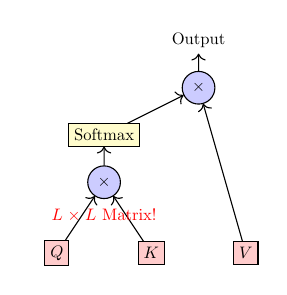
\begin{tikzpicture}[scale=0.6, transform shape]
                \node[draw, fill=red!20] (q) at (0,0) {$Q$};
                \node[draw, fill=red!20] (k) at (2,0) {$K$};
                \node[draw, fill=red!20] (v) at (4,0) {$V$};
                \node[draw, circle, fill=blue!20] (mul) at (1,1.5) {$\times$};
                \node[draw, rectangle, fill=yellow!20] (soft) at (1,2.5) {Softmax};
                \node[draw, circle, fill=blue!20] (mul2) at (3,3.5) {$\times$};
                \node (out) at (3,4.5) {Output};
                
                \draw[->] (q) -- (mul);
                \draw[->] (k) -- (mul);
                \draw[->] (mul) -- (soft);
                \draw[->] (soft) -- (mul2);
                \draw[->] (v) -- (mul2);
                \draw[->] (mul2) -- (out);
                
                \node[text width=3cm, align=center, red] at (1, 0.8) {$L \times L$ Matrix!};
            \end{tikzpicture}
        \end{column}
    \end{columns}
\end{frame}

% Slide 2b - Motivation Part 2
\begin{frame}{The Goal: The Ideal Sequence Model}
    \textbf{We want a model that combines the best of all worlds:}
    
    \vspace{0.5cm}
    \begin{table}
        \centering
        \begin{tabular}{lccc}
            \toprule
            \textbf{Feature} & \textbf{RNNs} & \textbf{Transformers} & \textbf{Ideal SSM} \\
            \midrule
            Training Parallelism & No & \textbf{Yes} & \textbf{Yes} \\
            Inference Speed & \textbf{$O(1)$} & $O(L)$ & \textbf{$O(1)$} \\
            Long-Range Dependencies & Weak & \textbf{Strong} & \textbf{Strong} \\
            Scalability to 1M+ tokens & No & No & \textbf{Yes} \\
            \bottomrule
        \end{tabular}
    \end{table}
    
    \vspace{0.5cm}
    \textbf{Core Objective:} Linear-time sequence modeling with Transformer-level performance on dense modalities (Language).
\end{frame}

% Slide 3 - SSM Foundation
\begin{frame}{The Foundation: Continuous State Space Models}
    SSMs map input $x(t)$ to output $y(t)$ via latent state $h(t)$.
    
    \begin{columns}
        \begin{column}{0.5\textwidth}
            \textbf{Continuous-Time LTI System:}
            \begin{align*}
                h'(t) &= A h(t) + B x(t) \\
                y(t) &= C h(t)
            \end{align}
            \begin{itemize}
                \item $h(t) \in \mathbb{R}^N$: Compressed History
                \item $A \in \mathbb{R}^{N \times N}$: Evolution Matrix
            \end{itemize}
        \end{column}
        \begin{column}{0.5\textwidth}
            % TikZ Diagram for SSM
            \begin{tikzpicture}[node distance=1.5cm, auto, >=latex']
                \node [draw, rectangle, fill=green!20, minimum height=1.5cm] (A) {$A$};
                \node [coordinate, left=of A] (input) {};
                \node [coordinate, right=of A] (output) {};
                \node [above] at (input) {$x(t)$};
                \node [above] at (output) {$y(t)$};
                
                \draw[->, thick] (input) -- node[above] {$B$} (A);
                \draw[->, thick] (A) -- node[above] {$C$} (output);
                \draw[->, thick] (A) edge [loop above] node {$h(t)$} (A);
            \end{tikzpicture}
        \end{column}
    \end{columns}
    
    \vspace{0.3cm}
    Usually, $N \approx 16$ (Small state). The matrix $A$ dictates how memory evolves.
\end{frame}

% Slide 4 - Discretization
\begin{frame}{Discretization: Continuous $\to$ Discrete}
    To process tokenized text, we must discretize using a step size $\Delta$.
    
    \vspace{0.3cm}
    \textbf{Zero-Order Hold (ZOH):}
    \begin{equation*}
        \overline{A} = \exp(\Delta A), \quad \overline{B} = (\Delta A)^{-1}(\exp(\Delta A) - I) \cdot \Delta B
    \end{equation}
    
    \vspace{0.3cm}
    \textbf{Two Modes of Computation:}
    \begin{enumerate}
        \item \textbf{Recurrent Mode (Inference):} $h_k = \overline{A} h_{k-1} + \overline{B} x_k$. Efficient autoregressive generation ($O(1)$).
        \item \textbf{Convolutional Mode (Training):} $y = x * \overline{K}$. Parallelizable via FFT ($O(L \log L)$).
    \end{enumerate}
\end{frame}

% Slide 5 - S4 and HiPPO
\begin{frame}{S4: Solving the Long-Range Memory Problem}
    Standard SSMs struggle to remember long history. \textbf{S4 (Structured State Space)} solves this.
    
    \vspace{0.3cm}
    \begin{columns}
        \begin{column}{0.6\textwidth}
            \textbf{Key Innovation: HiPPO Initialization}
            \begin{itemize}
                \item \textbf{HiPPO (High-order Polynomial Projection Operator):} A mathematical framework to approximate a continuous function history using orthogonal polynomials.
                \item \textbf{Mechanism:} Initializes matrix $A$ specifically to compress history optimally.
                \item \textbf{Result:} Prevents vanishing gradients; enables dependencies over $>10,000$ steps.
            \end{itemize}
        \end{column}
        \begin{column}{0.4\textwidth}
            \centering
            \footnotesize
            $$ A_{nk} = \begin{cases} (2n+1)^{1/2}(2k+1)^{1/2} & n > k \\ n+1 & n=k \\ 0 & n < k \end{cases} $$
            \textit{(HiPPO Matrix Example)}
        \end{column}
    \end{columns}
\end{frame}

% Slide 6 - Need for Selectivity
\begin{frame}{The Limitation of S4: Linear Time-Invariance (LTI)}
    \begin{block}{What is the LTI Limitation?}
        In S4, matrices $A, B, C$ and $\Delta$ are fixed (or learned statically). They do \textbf{not} change based on the current input token $x_t$.
    \end{block}
    
    \vspace{0.3cm}
    \textbf{Why is this critical for language?}
    \begin{itemize}
        \item \textbf{Language is Discrete:} A model needs to "reset" memory at a period, or "ignore" filler words (e.g., "ummm").
        \item \textbf{Content-Awareness:} Attention works because $Q, K$ interaction is input-dependent. LTI filters look at all inputs with the same "lens."
    \end{itemize}

    \vspace{0.3cm}
    \begin{center}
        \colorbox{lightblue!30}{%
            \parbox{0.6\textwidth}{%
                \centering
                \textbf{Solution:} Make parameters functions of input $x_t$.\\
                \textbf{LTI $\to$ LTV (Linear Time-Varying)}
            }
        }
    \end{center}
\end{frame}

% Slide 7 - S6 Mechanism
\begin{frame}{S6: The Selective State Space Model}
    \textbf{Mechanism:} Input $x_k$ generates the dynamics for step $k$.
    
    \begin{columns}
        \begin{column}{0.5\textwidth}
            \textbf{1. Selection Projections:}
            \begin{align*}
                B_k &= \text{Linear}_B(x_k) \\
                C_k &= \text{Linear}_C(x_k) \\
                \Delta_k &= \text{Softplus}(\text{Parameter} + \text{Linear}_\Delta(x_k))
            \end{align}
            \footnotesize{Note: $A$ remains static (helps optimization).}
        \end{column}
        \begin{column}{0.5\textwidth}
            \textbf{2. Discretization (Input-Dependent):}
            \begin{align*}
                \overline{A}_k &= \exp(\Delta_k A) \\
                \overline{B}_k &= (\Delta_k A)^{-1}(\exp(\Delta_k A) - I) \cdot \Delta_k B_k
            \end{align}
        \end{column}
    \end{columns}
    
    \vspace{0.5cm}
    \textbf{Intuition:}
    \begin{itemize}
        \item \textbf{Small $\Delta_k$:} Ignore input (keep state).
        \item \textbf{Large $\Delta_k$:} Focus on input (overwrite state).
        \item This allows \alert{Content-Based Reasoning} (Copying, Induction Heads).
    \end{itemize}
\end{frame}

% Slide 8 - S6 Discretization Details
\begin{frame}{Discretization Details \& Stability}
    Why project $B$ and $\Delta$ separately?
    
    \begin{itemize}
        \item \textbf{$\Delta$ (Timescale):} Controls the balance between "remembering" and "current input". Input-dependent $\Delta$ allows the model to compress or expand time based on information density.
        \item \textbf{$B, C$ (Interaction):} Control how much the input modifies the state and how much state affects the output.
    \end{itemize}
    
    \vspace{0.5cm}
    \textbf{Computational Implication:}
    Since $\overline{A}_k$ varies with time $k$, we \alert{cannot} use Convolution ($K$ is not fixed). We lose the $O(L \log L)$ FFT trick.
\end{frame}

% Slide 9a - The Training Challenge
\begin{frame}{The Training Challenge}
    We gained \textbf{Selectivity} (Content-Awareness), but we lost \textbf{Convolution}.
    
    \vspace{0.5cm}
    \begin{itemize}
        \item \textbf{Naive Recurrence:} $h_k = \overline{A}_k h_{k-1} + \overline{B}_k x_k$
        \item This is sequential. On a GPU, calculating $h_k$ requires waiting for $h_{k-1}$.
        \item For sequence length $L$, this takes $O(L)$ sequential steps.
        \item \textbf{Result:} Very slow training compared to Transformers (which train in parallel).
    \end{itemize}
    
    \vspace{0.5cm}
    \centering
    \alert{How do we train LTV models efficiently?}
\end{frame}

% Slide 9b - Parallel Scan Solution
\begin{frame}{Solution: The Parallel Scan}
    We can parallelize recurrence using the \textbf{Associative Property}.
    
    \vspace{0.3cm}
    \textbf{Concept:}
    Instead of calculating $h_1 \to h_2 \to h_3 \dots$, we define an operator $\circ$.
    \begin{equation*}
        (A_j, B_j) \circ (A_i, B_i) = (A_j A_i, A_j B_i + B_j)
    \end{equation}
    
    \vspace{0.2cm}
    \textbf{Tree Reduction:}
    We can compute the cumulative states in $O(\log L)$ steps using a tree structure.
    
    \begin{center}
    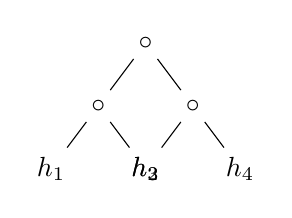
\begin{tikzpicture}[level distance=1cm, sibling distance=1.5cm, scale=0.8]
      \node {$\circ$}
        child {node {$\circ$}
          child {node {$h_1$}}
          child {node {$h_2$}}
        }
        child {node {$\circ$}
          child {node {$h_3$}}
          child {node {$h_4$}}
        };
    \end{tikzpicture}
    \end{center}
    
    This restores \alert{Parallel Training} for Selective SSMs.
\end{frame}

% Slide 10 - The Mamba Architecture
\begin{frame}{From S6 to Mamba: The Architecture}
    \textbf{S6 is just the inner layer.} Mamba is the Neural Network Block.
    
    \begin{columns}
        \begin{column}{0.5\textwidth}
            \textbf{Motivation:}
            \begin{itemize}
                \item S6 needs to be wrapped in a stable block (like Multi-Head Attention is wrapped in Transformer blocks).
                \item Mamba simplifies the H3 architecture and combines it with the MLP block.
            \end{itemize}
            
            \textbf{Structure:}
            \begin{itemize}
                \item Expand input dimension ($D \to 2D$).
                \item Branch 1: Convolution + S6.
                \item Branch 2: Gating (SiLU).
                \item Element-wise Product (Gating).
            \end{itemize}
        \end{column}
        \begin{column}{0.5\textwidth}
            % TikZ Diagram for Mamba Block
            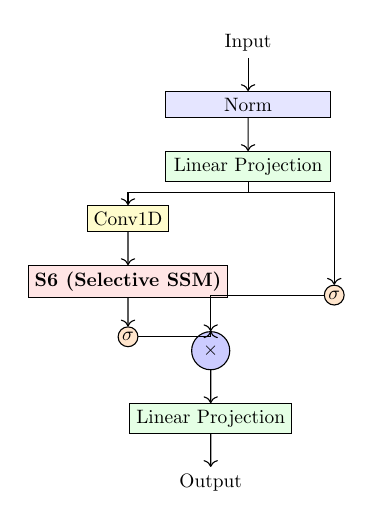
\begin{tikzpicture}[node distance=0.6cm, auto, scale=0.7, transform shape]
                \node (input) {Input};
                \node [draw, rectangle, fill=blue!10, below=of input, minimum width=3cm] (norm) {Norm};
                \node [draw, rectangle, fill=green!10, below=of norm, minimum width=3cm] (proj) {Linear Projection};
                
                % Branch 1
                \node [draw, rectangle, fill=yellow!20, below left=of proj, xshift=0.5cm] (conv) {Conv1D};
                \node [draw, rectangle, fill=red!10, below=of conv] (ssm) {\textbf{S6 (Selective SSM)}};
                \node [draw, circle, fill=orange!20, inner sep=1pt] (act1) at ($(ssm)+(0,-1)$) {$\sigma$};
                
                % Branch 2
                \node [draw, circle, fill=orange!20, inner sep=1pt, below right=of proj, xshift=-0.5cm, yshift=-1.5cm] (act2) {$\sigma$};
                
                % Merge
                \node [draw, circle, fill=blue!20, below=of ssm, xshift=1.5cm] (mul) {$\times$};
                \node [draw, rectangle, fill=green!10, below=of mul] (outproj) {Linear Projection};
                \node [below=of outproj] (out) {Output};
                
                \draw[->] (input) -- (norm);
                \draw[->] (norm) -- (proj);
                \draw[->] (proj.south) -- ++(0,-0.2) -| (conv.north);
                \draw[->] (proj.south) -- ++(0,-0.2) -| (act2.north);
                \draw[->] (conv) -- (ssm);
                \draw[->] (ssm) -- (act1);
                \draw[->] (act1) -| (mul);
                \draw[->] (act2) -| (mul);
                \draw[->] (mul) -- (outproj);
                \draw[->] (outproj) -- (out);
            \end{tikzpicture}
        \end{column}
    \end{columns}
\end{frame}

% Slide 11 - HW Optimization
\begin{frame}{Hardware Optimization: Why it matters}
    \textbf{The Bottleneck:} In modern GPUs, \alert{Memory Bandwidth} (moving data) is slower than Compute (FLOPs).
    
    \vspace{0.3cm}
    \textbf{The Kernel Fusion Solution:}
    \begin{itemize}
        \item Standard PyTorch: Read $A, B$ from HBM $\to$ SRAM $\to$ Compute $\to$ Write HBM $\to$ Read HBM...
        \item \textbf{Mamba Fused Kernel:}
        \begin{itemize}
            \item Load parameters $(\Delta, A, B, C)$ once.
            \item Perform Discretization + Parallel Scan in fast SRAM.
            \item Only write the final result back to HBM.
        \end{itemize}
    \end{itemize}
    
    \vspace{0.3cm}
    \textbf{Result:} Training is not just theoretically linear $O(L)$, but empirically fast (faster than FlashAttention-2 for $L>2k$).
\end{frame}

% Slide 12 - Performance
\begin{frame}{Performance: Better Performance and Efficiency}
    Mamba outperforms Transformers of the same size and matches those $2\times$ larger.
    
    \vspace{0.3cm}
    \begin{columns}
        \begin{column}{0.5\textwidth}
            \textbf{Throughput (Inference):}
            \begin{itemize}
                \item \textbf{5x Higher Throughput} than Transformers.
                \item Constant memory usage (no KV cache).
            \end{itemize}
            
            \vspace{0.2cm}
            \textbf{Quality (Perplexity):}
            \begin{itemize}
                \item Mamba-3B matches Pythia-7B.
                \item Solves "Induction Heads" perfectly up to 1M tokens.
            \end{itemize}
        \end{column}
        \begin{column}{0.5\textwidth}
            \centering
            % Simplified Bar Chart
            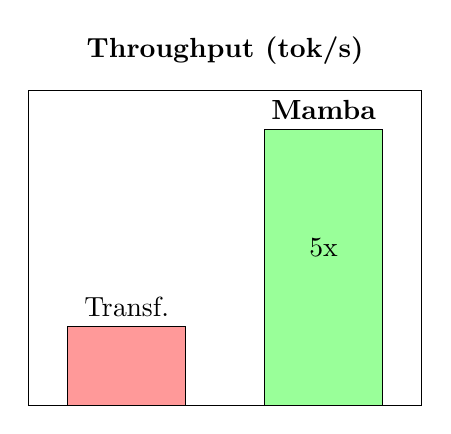
\begin{tikzpicture}
                \draw (0,0) -- (0,4) -- (5,4) -- (5,0) -- cycle;
                \node at (2.5, 4.5) {\textbf{Throughput (tok/s)}};
                
                % Transformer
                \draw[fill=red!40] (0.5,0) rectangle (2, 1);
                \node[above] at (1.25, 1) {Transf.};
                
                % Mamba
                \draw[fill=green!40] (3,0) rectangle (4.5, 3.5);
                \node[above] at (3.75, 3.5) {\textbf{Mamba}};
                
                \node at (3.75, 2) {5x};
            \end{tikzpicture}
            
            \vspace{0.2cm}
            \footnotesize{Source: Gu \& Dao (2023)}
        \end{column}
    \end{columns}
\end{frame}

% Slide 13 - Comparison Table
\begin{frame}{Comparison Summary}
    \small
    \begin{table}
        \centering
        \begin{tabular}{@{}lccc@{}}
            \toprule
            \textbf{Feature} & \textbf{Transformer} & \textbf{S4 (LTI)} & \textbf{Mamba (S6)} \\
            \midrule
            Complexity (Train) & $O(L^2)$ & $O(L \log L)$ & $O(L \log L)$ \\
            Complexity (Infer) & $O(L)$ & $O(1)$ & \alert{$O(1)$} \\
            Selectivity & \textbf{Yes} & No & \textbf{Yes} \\
            Implementation & MatMul & FFT & Scan \\
            Language Quality & High & Low & \textbf{High} \\
            \bottomrule
        \end{tabular}
    \end{table}
    
    \centering
    \textbf{Key Takeaway:} Mamba bridges the gap: Efficiency of RNNs + Power of Attention.
\end{frame}

% Slide 14 - Applications
\begin{frame}{Practical Applications}
    Where does Mamba excel?
    \begin{itemize}
        \item \textbf{Long-Context NLP:} Documents $>100k$ tokens where Attention OOMs.
        \item \textbf{Genomics:} DNA modeling (Millions of base pairs) [Nguyen et al., 2023].
        \item \textbf{Audio/Speech:} Waveform generation (Time-continuous data).
        \item \textbf{Time-Series:} Financial or Weather forecasting with long history.
    \end{itemize}
    
    \vspace{0.3cm}
    \footnotesize{
    References:\\
    Gu \& Dao, "Mamba: Linear-Time Sequence Modeling..." (2023)\\
    Nguyen et al., "HyenaDNA: Long-Range Genomic Sequence Modeling..." (2023)
    }
\end{frame}

% Slide 15 - Open Questions
\begin{frame}{Current Research \& Limitations}
    \textbf{Limitations:}
    \begin{itemize}
        \item \textbf{Implementation Barrier:} Requires custom CUDA kernels (Triton/C++).
        \item \textbf{Stability:} Harder to train than Transformers at massive scale ($>100B$).
    \end{itemize}
    
    \textbf{Active Research Areas:}
    \begin{itemize}
        \item \textbf{Selective A Matrix:} Can making $A$ input-dependent improve results? Currently, only $B, C, \Delta$ are selective.
        \item \textbf{Multimodality:} Extending 1D scans to 2D images (Vision Mamba) and 3D Video.
    \end{itemize}
\end{frame}

% Slide 16 - Mamba Variants
\begin{frame}{New Developments: Mamba Variants}
    Based on recent surveys (e.g., Wang et al., 2024), the architecture is evolving rapidly:
    
    \begin{itemize}
        \item \textbf{Vision Mamba (Vim) / VMamba:} Solves 2D spatial loss by scanning images in 4 directions (Cross-Scan). Outperforms ViT in efficiency.
        \item \textbf{Jamba (AI21):} Hybrid architecture. Interleaves Mamba layers with Transformer Attention layers.
            \begin{itemize}
                \item Benefits: High quality retrieval (Attention) + High throughput (Mamba).
            \end{itemize}
        \item \textbf{MambaByte:} Token-free language modeling (directly on bytes).
        \item \textbf{MoE-Mamba:} Mixture of Experts combined with SSMs for massive scale.
    \end{itemize}
\end{frame}

% Slide 17 - Adoption & Low Power
\begin{frame}{Adoption Status and Low-Power Future}
    \textbf{Current Adoption:}
    \begin{itemize}
        \item \textbf{Research:} High. Hundreds of variants in 2024.
        \item \textbf{Production:} Moderate but growing. \textit{Jamba} is a production-grade LLM.
    \end{itemize}
    
    \textbf{Low-Power/Edge Applications:}
    \begin{itemize}
        \item \textbf{Constant Memory:} Because inference memory is $O(1)$ (fixed state size), Mamba is ideal for embedded devices with limited RAM.
        \item \textbf{Battery Life:} Reduced compute for long-context generation saves energy compared to quadratic Attention.
        \item \textbf{Robotics:} Fast, recurrent processing suits real-time control loops.
    \end{itemize}
\end{frame}

% Slide 18 - Future Scope
\begin{frame}{Future Scope}
    \begin{itemize}
        \item \textbf{Replacement for Transformers?} Unlikely to fully replace, but "Hybrid" models (Jamba style) are likely the future of LLMs.
        \item \textbf{Hardware Accelerators:} New chips might be optimized for linear scans rather than just Matrix Multiplications.
        \item \textbf{Interpretability:} Understanding the state $h$ is harder than visualizing Attention maps. Tools are needed.
    \end{itemize}
    
    \vspace{0.5cm}
    \centering
    \Large \textbf{Conclusion:} Mamba is the most viable alternative to the Transformer in 5 years.
\end{frame}

\end{document}
```
